\chapter{Analysis and Design}
This chapter gives an overview of the overall system and explains the design choices made. Throughout the project, we explored various methods to implement a real-time augmented reality system for PWUs operating a wheelchair. Naturally, the structure and goals of the project have developed since the interim report, and we review the differences between the initial goals and final product .

\section{Design Overview}
As stated in the requirements, this project consists of three major components:
\begin{itemize}
	\item Human Detection and Direction (HDD)
	\item Object Mapping and Visualization (OMV)
	\item Reactive Control on ARTA
\end{itemize}

\begin{figure}[ht]
	\centering
	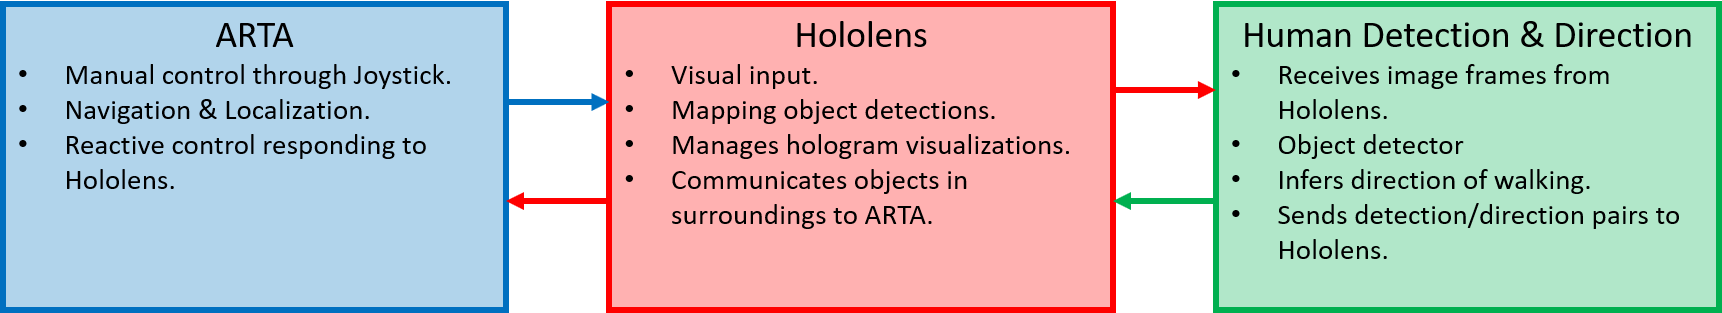
\includegraphics[width=1.0\linewidth]{img/chapter4_analysis/simpleSystemDiagram.png}
	\caption{Simplified high level system diagram}
	\label{fig:simplifiedHL}
\end{figure}

From a very high level view, we can map these requirements to the respective devices they will be operating on. The HDD system takes implements the object detection and human direction inference, while the Hololens is responsible for utilizing the spatial mapping to obtain world positions of the detections, as well as visualizing the detections. The powered wheelchair (ARTA), has manual input that is overridden by the reactive control system that is dependent upon the detections and mappings. The diagram in Figure. \ref{fig:simplifiedHL} shows an overview of the system, and shows that the Hololens acts as an intermediary between ARTA and the HDD.

\subsection{Hardware}

\begin{table}[ht]
	\centering
	\begin{tabular}{l|l|l|l|}
		\cline{2-4}
		& \multicolumn{1}{c|}{\textbf{ARTA}}                                                 & \multicolumn{1}{c|}{\textbf{Hololens}} & \multicolumn{1}{c|}{\textbf{HDD}}                              \\ \hline
		\multicolumn{1}{|l|}{\textbf{Hardware}}         & \begin{tabular}[c]{@{}l@{}}Powered Wheelchair \\ controlled by Laptop\end{tabular} & Hololens                               & \begin{tabular}[c]{@{}l@{}}Desktop PC \\ with GPU\end{tabular} \\ \hline
		\multicolumn{1}{|l|}{\textbf{Operating System}} & Ubuntu 16.04                                                                       & UWP                                    & Ubuntu 16.04                                                   \\ \hline
	\end{tabular}
	\caption{Hardware description of system}
	\label{tab:hardware}
\end{table}

Table. \ref{tab:hardware} summarises the hardware overall system is implemented on. The powered wheelchair, ARTA, is controlled by a laptop, which is responsible for the wheelchair speed, wheel rotations, navigation and localisation. The Hololens is a self contained augmented reality headset, running the Universal Windows Platform (UWP) operating system. Finally, the Human Detection \& Direction system is implemented on a desktop computer with a GTX 1050Ti GPU, allowing it to run real time object detectors.

\subsection{Communication}

\subsubsection{Robotic Operating System} Since the system spans multiple operating systems, we have chosen to utilize the Robotic Operating System (ROS) as a means of communication between the devices. ROS defines a \textit{node} as a process that performs a computation, and every node can be made of smaller nodes that perform specific computations that serve the needs of the parent node. 

\begin{figure}[ht]
	\centering
	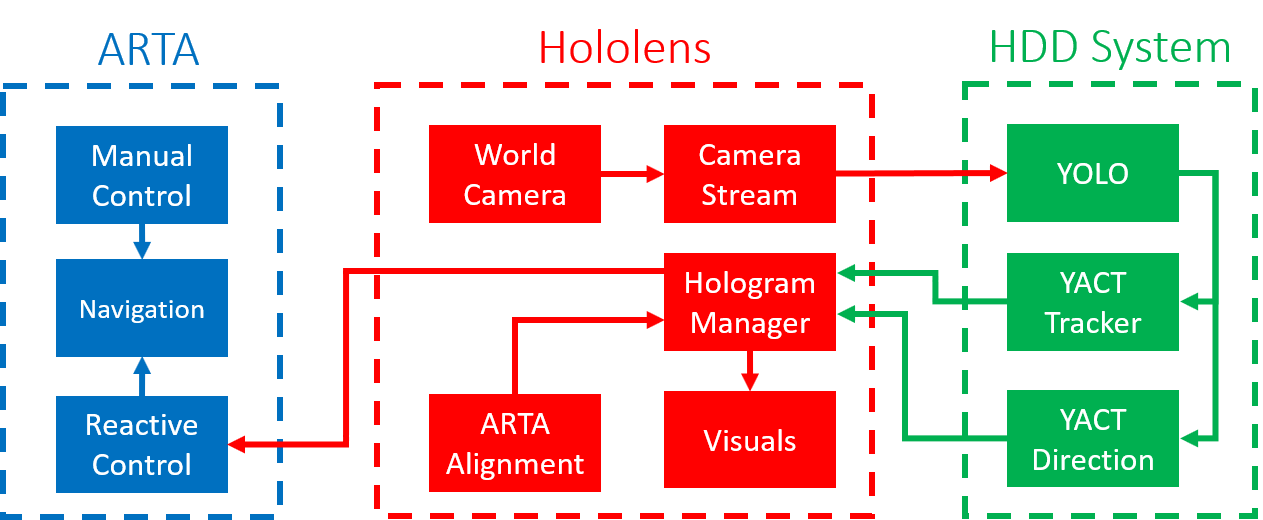
\includegraphics[width=1.0\linewidth]{img/chapter4_analysis/detailedSystemDiagram.png}
	\caption{System diagram detailing individual components}
	\label{fig:detailedHL}
\end{figure}

We can think of the three major systems as large ROS nodes that consists of smaller nodes that run individiual tasks, such as creating the camera stream, or detecting objects. We visualize the breakdown of the system into nodes in Figure. \ref{fig:detailedHL}.

\paragraph{ROS Topics} Nodes in ROS communicate with one another by publishing data in the form of \textit{messages} which get broadcasted over a \textit{topic}. Nodes can subscribe to topics that they want to receive data from. This method allows for nodes running on different devices to communicate with each other, regardless of the operating system, without even realizing that the nodes are running on a seperate computer.

\section{Human Detection \& Direction System}

\subsection{Breakdown}

\section{Hololens}
\subsection{Breakdown}

\section{ARTA}
\subsection{Breakdown}


